

%%%%%%%%%%%%%%%%%%%%%%%%%%%%%%%%%%%%%%%%%%%%%%%%%%%%%%%%%%%%%%%%%%%%%%%%%%%%%%
\section{Regular mode: RUN105038}
\subsection{Time distribution and occupancy}
Similar to the approach outlined in Section \ref{over}, the first distribution to see was the time distribution of number of hits in channels of the first and second FPGA. Given that we are not operating in an overflow mode, our observations reveal a uniform temporal distribution for both cases, as we expected.
\begin{figure}[H]
  \hspace{-0.5in}
  \begin{tikzpicture}
    \node[anchor=south west,inner sep=0] at (0,0.) {
      % \node[shift={(0 cm,0.cm)},inner sep=0,rotate={90}] at (0,0) {}
      % \makebox[\textwidth][c] {
      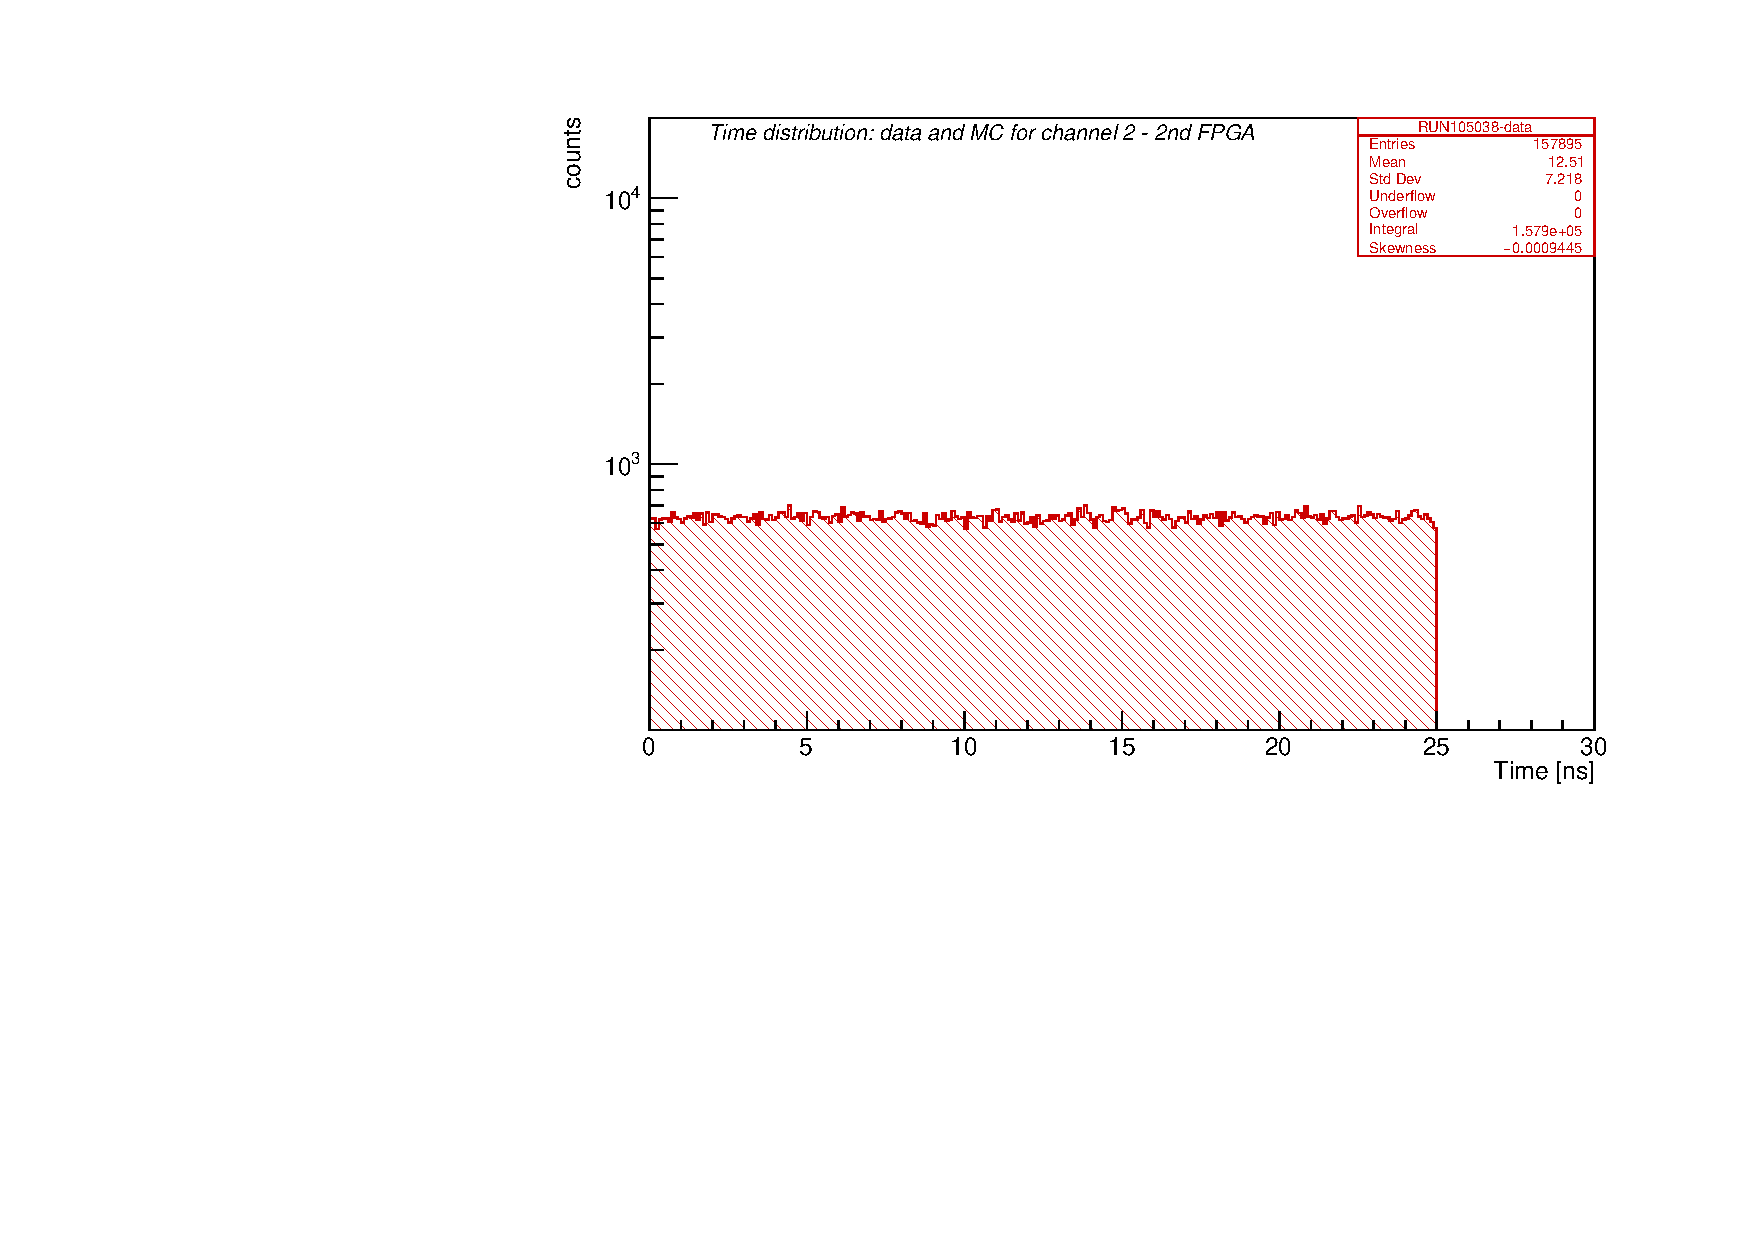
\includegraphics[width=0.5\textwidth]{figures/pdf/figure_00012_timedistr_roc_simulation_ch2_105038}
      % }
    };
    \node[anchor=south west,inner sep=0] at (10,0.) {
      % \node[shift={(0 cm,0.cm)},inner sep=0,rotate={90}] at (0,0) {}
      % \makebox[\textwidth][c] {
      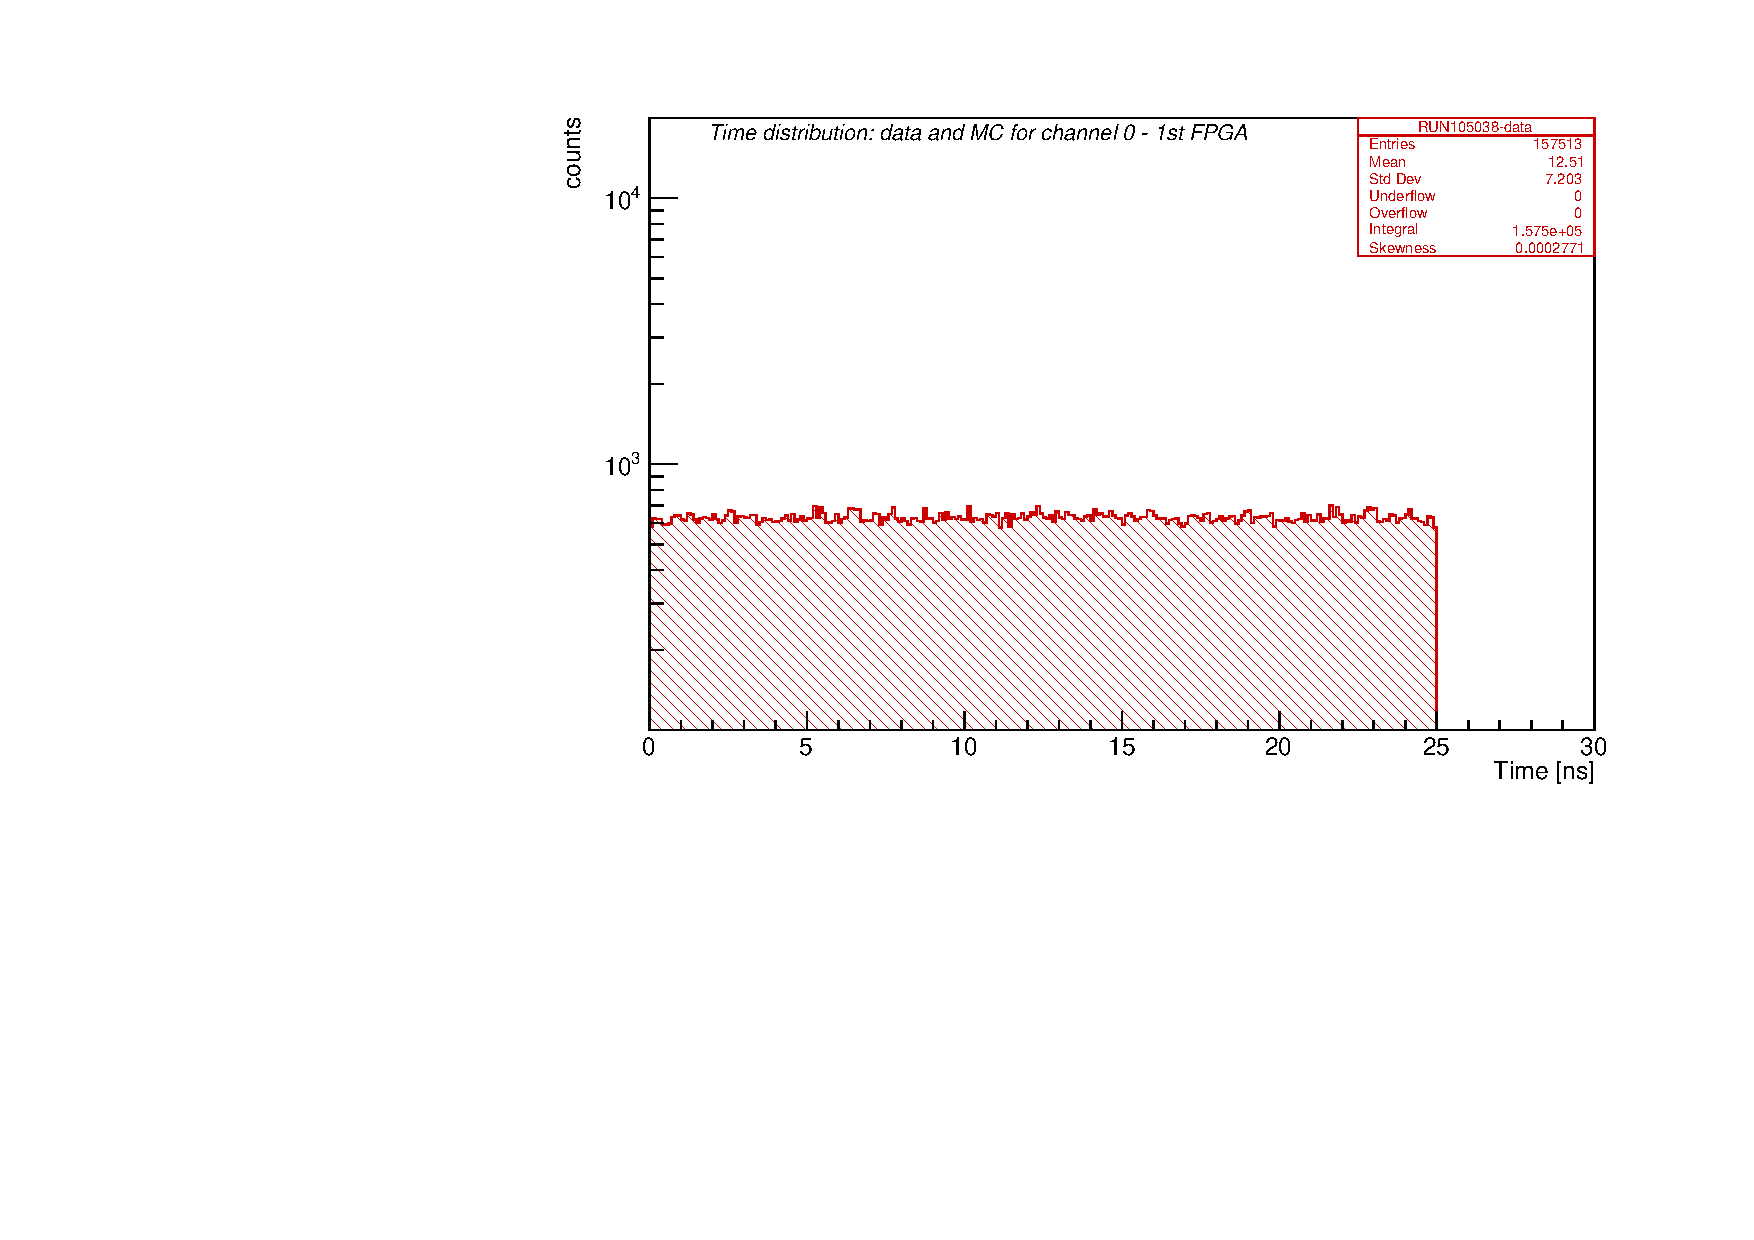
\includegraphics[width=0.5\textwidth]{figures/pdf/figure_00001_timedistr_roc_simulation_10538}
      % }
    };
  \end{tikzpicture}
  \caption{
    \label{fig:4}
    right: First FPGA's channel time distribution, left: Second FPGA's channel time distribution.
  }
\end{figure}
The time distibution can beeasily understood by watching the occupancy plot in Fig.\ref{fig:5}. The occupancy is a uniform distribution, as we expected operating in a non-overflow mode. Channels ordering is the readout order.
\begin{figure}[!h]
\centering
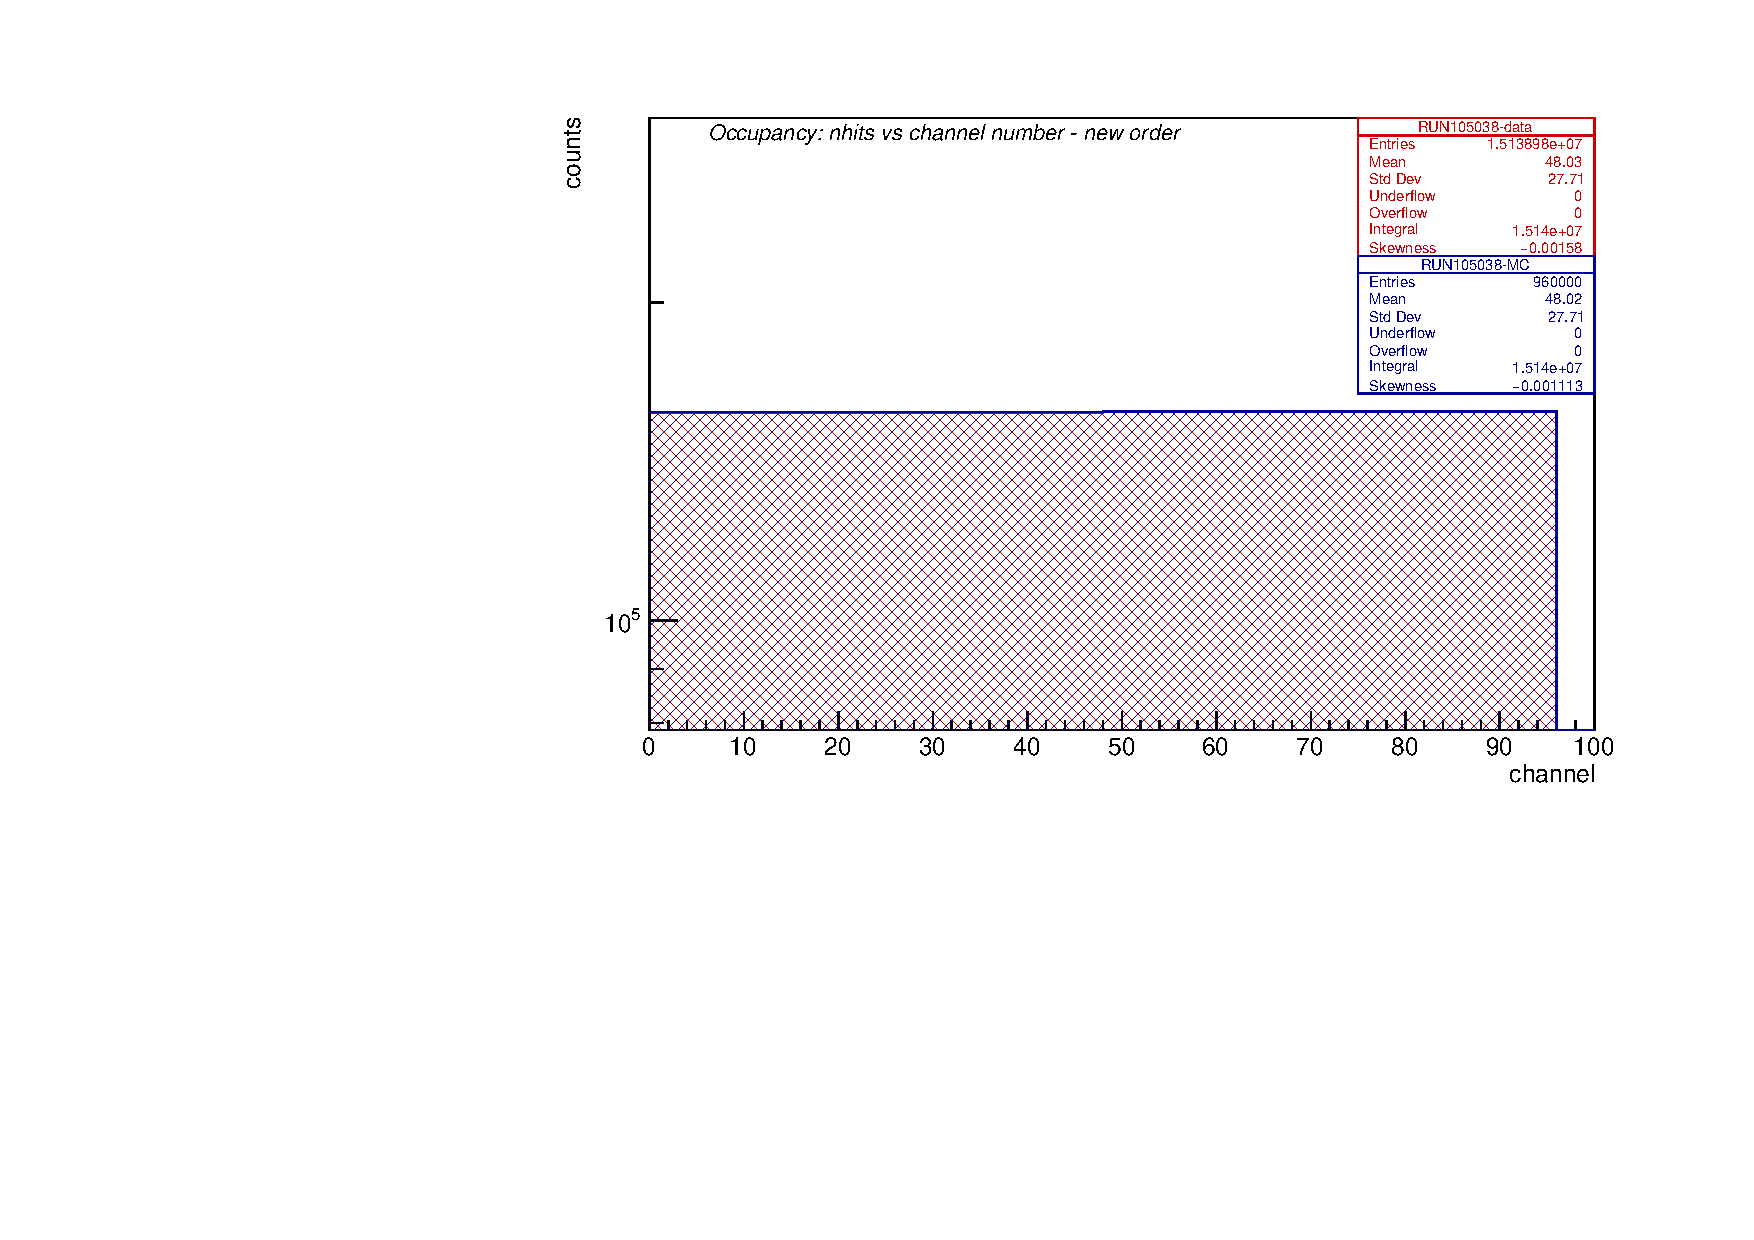
\includegraphics[width =0.8\textwidth]{figures/pdf/figure_00002_nhitsvschannel_roc_simulation_2}
\caption{Occupancy: number of hits versus channel in the underflow mode.}
\label{fig:5}
\end{figure}

\subsection{Number of hits}
As conclusion we can see in Fig. \ref{fig:6}, the main aspect of non-overflow mode: the number of hits are not anymore peaked in 255 and so this reflects in the fact that the number of bytes are not always the same.
\begin{figure}[!h]
\centering
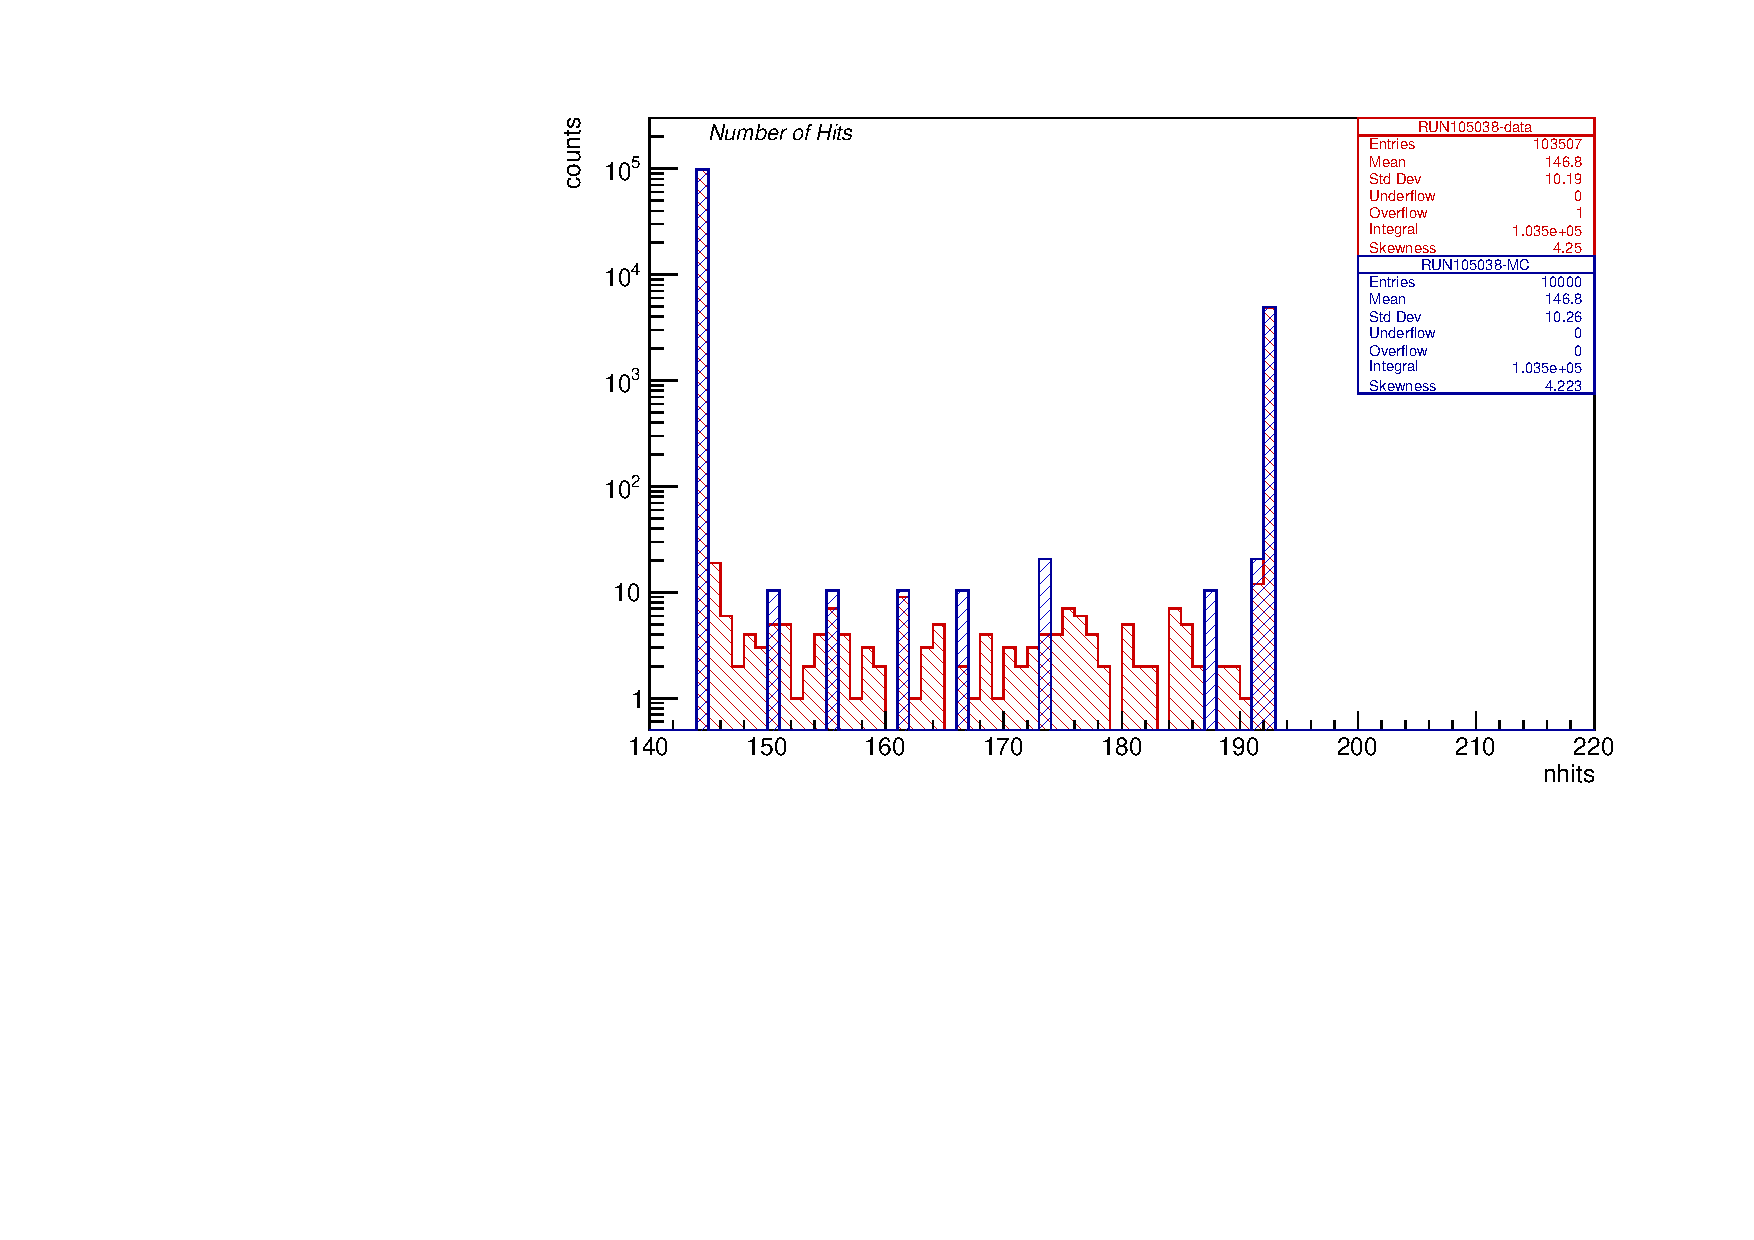
\includegraphics[width =0.8\textwidth]{figures/pdf/figure_00009_nhits_105038}
\caption{Number of hits distribution.}
\label{fig:6}
\end{figure}










%%% Local Variables:
%%% mode: latex
%%% TeX-master: t
%%% End:
